
\documentclass[11pt,a4paper]{article}

% --- Encoding and typography ---
\usepackage[T1]{fontenc}
\usepackage[utf8]{inputenc}
\usepackage{lmodern}
\usepackage{microtype}

% --- Layout ---
\usepackage[a4paper,margin=1in]{geometry}
\usepackage{setspace}
\onehalfspacing

% --- Math, tables, figures ---
\usepackage{amsmath,amssymb}
\usepackage{booktabs}
\usepackage{graphicx}
\usepackage{subcaption}
\usepackage{siunitx}
\usepackage{rotating}
\usepackage{url}
% Long repository paths: also allow breaks after underscores.
\expandafter\def\expandafter\UrlBreaks\expandafter{\UrlBreaks\do\_}

% --- References (simple and journal-compatible baseline) ---
\usepackage[numbers,sort&compress]{natbib}

\title{Unifying Search Paradigms using optDSL}
\author{
  Michael Bögl
}
\date{\today}

\begin{document}
\maketitle

\begin{abstract}
In practical combinatorial optimization, solver-paradigm decisions are frequently made at an early project stage.
Such early commitments constrain subsequent modeling choices and can render later paradigm changes technically and organizationally costly.
This report addresses that limitation through a workflow that enables paradigm switching over the full project lifecycle.
The workflow is based on \texttt{optDSL} as a shared problem representation, leveraging its existing MiniZinc translation and extending the same representation with a Large Neighborhood Search (LNS) backend.
We detail the LNS design, including operator profiles, initialization strategies, and restart mechanisms, and evaluate the approach on benchmark instances from multiple problem classes.
Under fixed iteration and time budgets, we compare LNS-based heuristic search with a MiniZinc-based exact baseline on identical \texttt{optDSL} instances, and we further demonstrate practical applicability on a real-world use case within an extensible, model-driven optimization workflow.
\end{abstract}

\section{Introduction}
Combinatorial optimization practitioners routinely face a tension between solution quality, computation time, and implementation effort.
In many real projects, model requirements evolve over time, while the decision for a solver paradigm is made early and is difficult to revise later.
This creates a methodological lock-in that reduces both technical flexibility and practical efficiency.

Exact methods provide strong guarantees, most notably provable optimality and bounds on solution quality.
These properties are essential when results must be validated formally.
However, exact methods also exhibit well-known drawbacks.
Their computational cost can grow prohibitively on large or highly constrained instances, so that no acceptable solution may be available within practical time limits.
Their performance is sensitive to formulation quality, solver configuration, and available hardware, which makes results difficult to predict in advance.
Moreover, tight integration with a specific solver technology increases the engineering cost of model changes and rapid iteration.

Heuristic and metaheuristic methods occupy the opposite end of this trade-off.
They typically deliver good solutions quickly, scale to large instances, and can exploit domain structure through tailored search strategies.
This makes them attractive under strict runtime limits or in settings with frequent re-optimization.
Their drawbacks mirror their strengths: they provide no global optimality guarantees and usually no quality bounds, so the gap to the optimum remains unknown.
Their performance depends strongly on design choices such as operators, initialization, restart policies, and parameter settings, and a configuration that works well for one problem class may transfer poorly to another.
Consequently, substantial development and tuning effort is often required before a heuristic becomes reliable in practice.

Neither paradigm dominates the other; their strengths and weaknesses are largely complementary.
Which paradigm is preferable typically changes over the course of a project, for example when instance sizes grow, when time budgets shrink, or when formal quality guarantees become necessary.
This observation motivates a unifying approach in which the problem is modeled once and the solution paradigm remains exchangeable.

\texttt{optDSL}, a Python-inspired domain-specific language for describing optimization problems, provides such a unifying representation.
A single \texttt{optDSL} model can be dispatched to conceptually different backends:
an exact backend, currently realized through a translation to the constraint modeling language MiniZinc and its portfolio of solvers, and
a heuristic backend, currently realized through a Large Neighborhood Search (LNS) framework that operates directly on \texttt{optDSL} decision variables.
Because both backends consume identical problem descriptions, users can defer the paradigm decision, switch paradigms as project requirements evolve, and compare both paradigms under a common protocol without re-modeling.
A single \texttt{optDSL} model is fed through an importer into two parallel pipelines, one deriving the MiniZinc representation for exact solvers and one operating directly on the \texttt{optDSL} decision variables inside the LNS framework.
Beyond this dispatch view, the architecture admits a forward-looking perspective, illustrated in Figure~\ref{fig:optdsl-validation}: a solution that the LNS backend writes back in \texttt{optDSL} format can be re-injected into the exact pipeline, where the MiniZinc representation and its solvers are used to validate and improve the solution and to derive quality bounds. This closes the loop between heuristic and formal optimization within one consistent, model-centric workflow.
In the figure, the dashed line together with the gray-shaded area marks this feedback loop (writing a solution back in \texttt{optDSL} format and passing it to the exact backend for validation and improvement); this step is performed outside the scope of the present technical report, which provides the component optimizers but not yet an automated orchestration of the loop.
The blue box, by contrast, denotes the LNS-based heuristic part; it is the component that this report evaluates, and its full integration into the feedback loop is intended to be automated in subsequent work.

\begin{figure}[t]
\centering
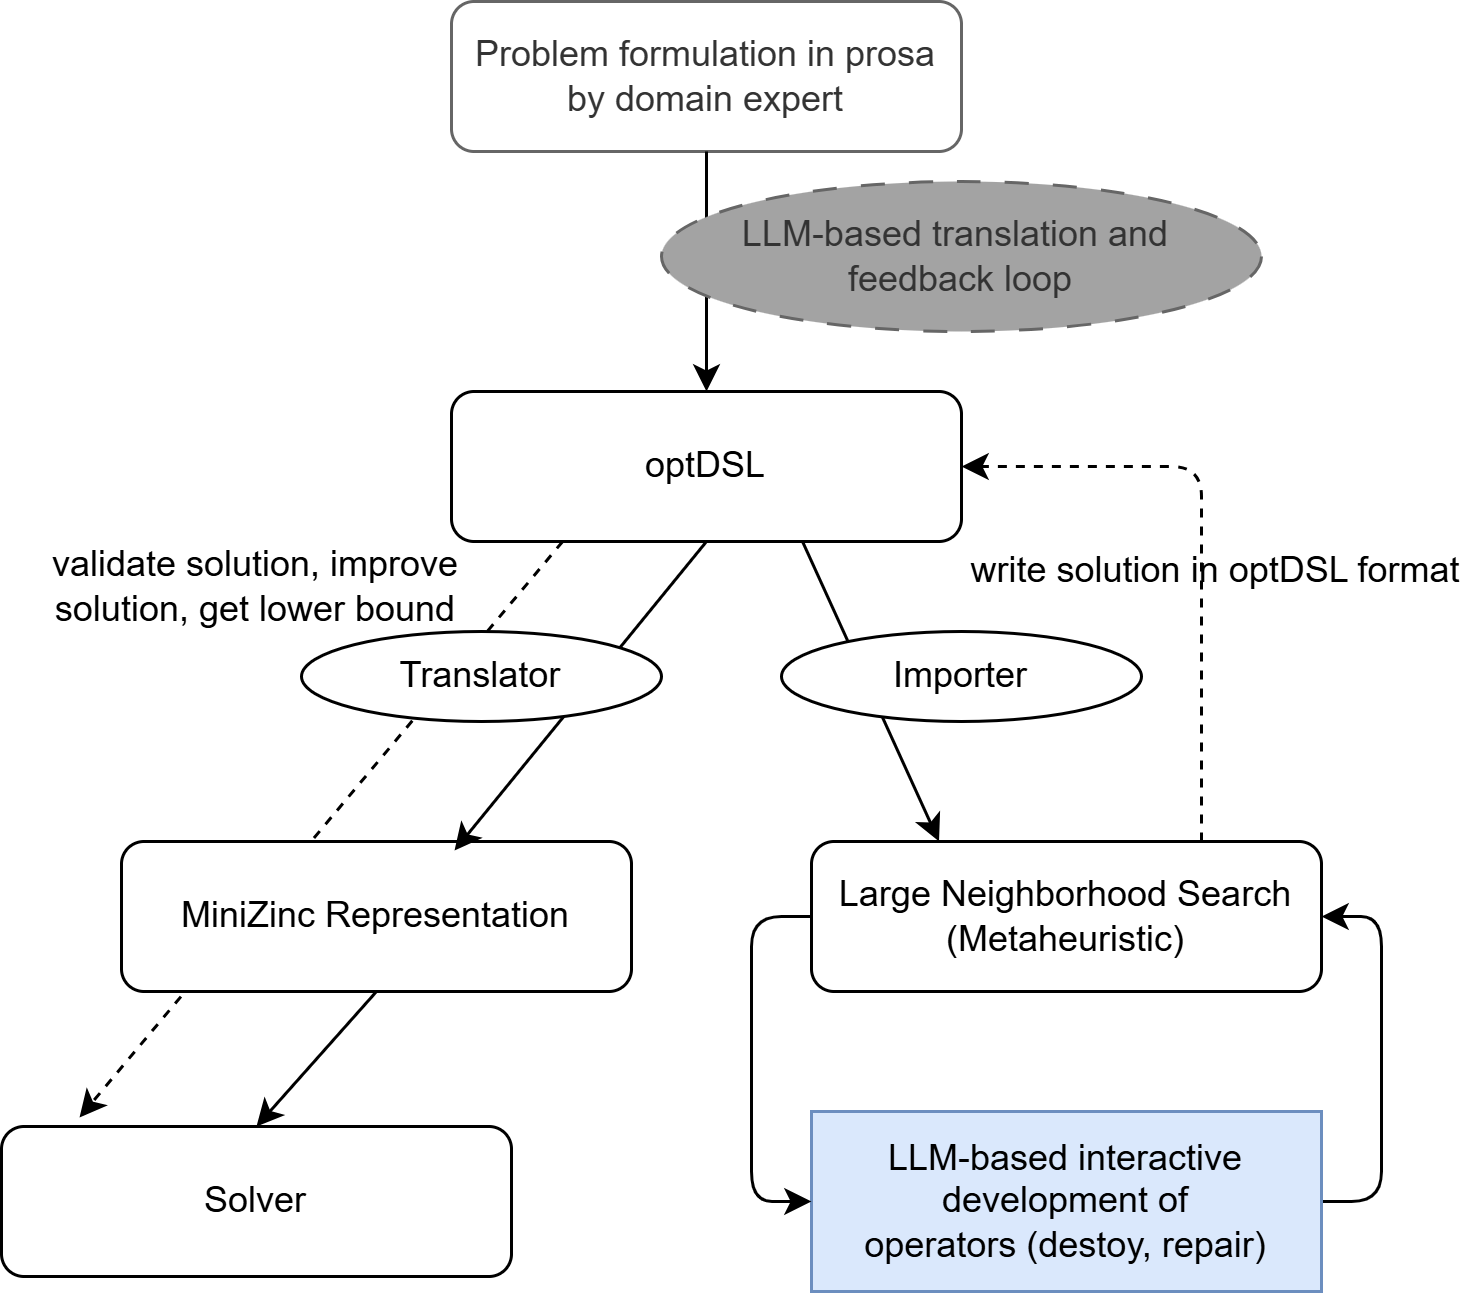
\includegraphics[width=0.6\textwidth]{optDSL_validation.drawio.png}
\caption{Perspective of the unifying workflow. The dashed line and the gray-shaded area mark the loop in which a solution is written back in \texttt{optDSL} format and passed to the exact backend for validation and improvement; this step is performed outside the scope of the present technical report. The blue box denotes the LNS-based heuristic part, which is intended to be automated in subsequent work.}
\label{fig:optdsl-validation}
\end{figure}

This report focuses on the design and evaluation of the LNS backend within this unified architecture.

We describe the implemented operator profiles, initialization strategies, and restart mechanisms, and evaluate the resulting search behavior on benchmark instances from multiple problem classes against the MiniZinc-based exact backend on identical \texttt{optDSL} instances.
The objective is twofold: to study how far adaptive LNS design can close the quality gap under fixed compute budgets, and to demonstrate the practical value of a model-centric workflow in which the solver strategy can be revised throughout the project lifecycle.

\section{Related Work}
Research on combinatorial optimization has increasingly moved from a strict exact-versus-heuristic dichotomy toward hybrid algorithms that combine the strengths of both paradigms.
In exact optimization, rich modeling languages and solver portfolios have improved accessibility and reproducibility, with MiniZinc becoming a standard interface for expressing models independently of the backend solver \citep{nethercote2007minizinc,stuckey2014minizinc}.
In parallel, neighborhood-based metaheuristics evolved from problem-specific local search to large-scale destroy-and-repair frameworks, where very large moves can be explored while preserving feasibility through structured repair \citep{shaw1998lns,ropke2006alns,pisinger2010lns,pisinger2019lns}.

An important algorithmic line that narrows the quality-runtime gap is the use of exact neighborhoods or exact reasoning inside heuristic search loops.
In mixed-integer optimization, local branching and relaxation-induced neighborhoods are representative bridge mechanisms: they constrain search to a promising region that can still be solved (approximately or exactly) by mathematical programming machinery \citep{fischetti2003localbranching,danna2005rin}.
The same principle appears in CP-LNS workflows, where exact propagation and constraint reasoning guide neighborhood repair, while the outer search remains heuristic and anytime \citep{shaw1998lns,pisinger2010lns,pisinger2019lns}.
Conceptually, these methods trade global proof guarantees for faster high-quality improvement, but recover part of exact-method robustness through bounded or solver-driven subproblems.

For routing, this bridge perspective is particularly visible in VRP and VRPTW.
Benchmark culture and instance standardization (e.g., Solomon and later CVRPLIB developments) enabled fair comparisons between exact, heuristic, and hybrid methods under shared protocols \citep{solomon1987vrptw,toth2014vrp,uchoa2017cvrplib}.
ALNS variants in this domain demonstrate that adaptive operator selection can substantially reduce the performance gap to exact baselines on larger instances where full proofs are expensive \citep{ropke2006alns,pisinger2010lns,pisinger2019lns}.

For packing and scheduling, the same pattern recurs with different primitives.
In two-dimensional bin packing, exact bounds and formulations are often paired with constructive and improvement heuristics in matheuristic pipelines \citep{lodi2002twodimensional,hopper2001genetic,hopper2001ejor,berkey1987,wang1983}.
In job shop scheduling, classic methods such as shifting bottleneck and tabu-search-based improvements can be interpreted as structured relax-and-improve strategies that inject stronger local reasoning than pure black-box metaheuristics \citep{adams1988shifting,taillard1993benchmarks,jain1999jssp,lawrence1984,applegate1991,storer1992}.
Across these classes, the literature suggests that performance gains arise when heuristic diversification is coupled with model-aware intensification.

A prerequisite for such cross-paradigm studies is a shared problem representation that both exact and heuristic solvers can consume.
optDSL addresses this need: it is a Python-inspired domain-specific language for formulating optimization problems, and a translation from optDSL to MiniZinc has been described and published \citep{delrio2026optdsl}, enabling optDSL instances to be solved by any MiniZinc-compatible backend solver.
The present report builds directly on that work.
Rather than proposing a new modeling language or a new translation pipeline, it uses the existing optDSL representation and MiniZinc translation as a foundation and contributes an experimental study that runs LNS-based heuristic search and MiniZinc-based exact solving on the same optDSL instances.
This enables an apples-to-apples comparison of how much algorithmic gap can be closed through shared instance engineering and adaptive neighborhood design across multiple problem classes, within the bridge-algorithm tradition described above.

\section{Method}
\subsection{optDSL Representation}
All benchmark instances are provided as standalone \texttt{optDSL} models
in which data, decision variables, constraints, and the objective form a
single self-contained file.
Syntactically, an \texttt{optDSL} model is a Python-inspired DSL
\citep{delrio2026optdsl}: scalar and array data are declared as typed
constants (e.g.\ \texttt{DSList(N, DSInt())} for integer arrays), decision
variables are declared with an explicit finite domain, feasibility
constraints are written as \texttt{assert} statements over (potentially
nested) loops and arithmetic, and the objective is declared as a final
\texttt{minimize(objective)} statement.
Because both backends consume exactly this file---the exact backend through
the translation to MiniZinc \citep{delrio2026optdsl}, the LNS backend
directly on the declared decision variables---no re-modeling is required
when switching between them.
We now summarize the model structure for the three main benchmark classes;
each relies on linear arithmetic over bounded integer domains, which keeps
the MiniZinc translation straightforward.

\textbf{Two-dimensional bin packing (2DBP).}
The model operates on three finite-domain decision-variable arrays
(\texttt{assignments}, \texttt{x\_positions}, \texttt{y\_positions}):
every item $i$ is assigned to a box $b$ and placed at a lower-left corner
$(x_i,y_i)$.
Feasibility is enforced by two constraint blocks: \texttt{all\_assigned}
ensures that each item receives exactly one box, and \texttt{no\_overlap}
first requires that each item fits within the dimensions of its selected
box and then requires, for any two items in the same box, that they do not
overlap in either the horizontal or the vertical direction.
The objective counts the number of distinct boxes in use and is minimized.
The converted benchmark instances live under
\texttt{problem\_instances/2dbp/benchmarks/testset\_paper\_optdsl/} and
contain 20 items on $10 \times 10$ bins.

\textbf{Capacitated vehicle routing (CVRP).}
Two semantically equivalent encodings are used, which illustrates that
\texttt{optDSL} permits representation choices tailored to the backend.
The \emph{arc-based} encoding declares a flat binary array
\texttt{arcs[v,i,j]} (with index $v\cdot n^2 + i\cdot n + j$), a binary
\texttt{vehicle\_used} indicator, and MTZ load variables \texttt{u}.
Constraints assert that every customer has in-degree and out-degree one
(\texttt{all\_customers\_visited}), that every used vehicle starts and ends
at the depot (\texttt{depot\_start\_end}), that flow is conserved at every
customer (\texttt{flow\_conservation}), that route demands respect the
vehicle capacity (\texttt{capacity\_constraints}), that no self-loops occur,
and that customer-only subtours are excluded through the Miller--Tucker--
Zemlin inequalities (\texttt{subtour\_elimination}); the objective sums the
traveled distance.
This encoding is used for the benchmark families distributed through the
CVRPLIB \citep{uchoa2017cvrplib} and is compatible with the MiniZinc
translation.
For the LNS backend on large instances we additionally use a
\emph{giant-tour} encoding with a permutation \texttt{tour} over customers
and a binary \texttt{cut\_after} array that marks route breaks at the
depot; constraints here are occurrence, route count, and a cumulative
capacity bound, and the objective inserts the depot detour at each cut.
This second encoding is intentionally LNS-oriented (it operates on the
permutation space of the route) and is not part of the MiniZinc baseline.

\textbf{Job shop scheduling (JSSP).}
The model declares finite-domain completion-time variables
\texttt{completion[j][op]} for every operation, bounded by
\texttt{MAX\_TIME}.
Two constraint blocks encode feasibility:
\texttt{precedence\_constraint} imposes the job-internal operation order
using the per-job \texttt{MACHINE\_SEQUENCE} and \texttt{PROCESSING\_TIMES},
and \texttt{no\_overlap\_constraint} asserts for every pair of operations
sharing a machine that one finishes before the other starts.
\texttt{PROCESSING\_TIMES[j][m]} is indexed by \emph{machine} id, while
\texttt{MACHINE\_SEQUENCE[j][op]} is indexed by \emph{operation} position, so
the processing time of operation \texttt{op} of job \texttt{j} is
\texttt{PROCESSING\_TIMES[j][MACHINE\_SEQUENCE[j][op]]}.
This convention is shared by the hand-written instances and by the LNS
operators, which read the same machine-indexed matrix.
The objective is the makespan, i.e.\ the maximum completion time over all
jobs.
Although the finite-domain completion-time formulation is a direct input
for the exact backend, the LNS repair operator reconstructs an equivalent
active schedule in the disjunctive space \citep{applegate1991}, so the
search is performed on the space of machine orders from which optimal
schedules are known to be recoverable.

Finally, next to the full benchmark sets, each class ships a number of
small hand-verified instances that serve as executable specifications of
the encodings above and as smoke tests for both backends, e.g.\ the
$2\times2$ and $5\times4$ JSSP models, the $E$-n13-k4 CVRP instance
(13 cities, 4 vehicles, known optimum 247), and the 20-item 2DBP test set.
% TODO: Decide whether to include one full listing of a tiny instance
% (e.g. jssp_2x2.dsl or E-n13-k4.dsl) as an illustrative figure.

\subsection{LNS Configuration}
The LNS backend instantiates the classical destroy-and-repair scheme of \citet{shaw1998lns} and combines it with the adaptive operator-selection and weight-update mechanism of ALNS \citep{ropke2006alns,pisinger2010lns,pisinger2019lns}.
Operator profiles are realized per problem class; in particular, the job-shop repair operator constructs active schedules in the spirit of \citet{applegate1991}.
% TODO: Describe destroy/repair operators, initialization, restart policy, and stopping criteria in detail.

\subsection{Evaluation Baselines}
The quality of the LNS backend is assessed against the exact MiniZinc-based
backend on identical \texttt{optDSL} instances.
On each instance, the exact backend either proves optimality or, when the
time limit is reached, yields a feasible incumbent together with an
optimality gap from its reported bound.
This provides two complementary baselines: reference (optimal) values for
small instances, and a certified lower bound to bound the achievable gap of
the heuristic on the larger benchmark families.
Where published optima or best-known values exist, they serve as an
additional independent reference
\citep{applegate1991,nowicki1996fast,taillard1993benchmarks,uchoa2017cvrplib,martello1998exact}.
% TODO: Describe comparative baselines used for evaluation (for example reference values, bounds, or external solvers).

\section{Experimental Setup}
\subsection{Benchmark Families}
We evaluate on benchmark families from four problem classes, chosen for their complementary structure, their prevalence in the literature, and the availability of reference solutions.

\textbf{Capacitated Vehicle Routing (CVRP).}
We use the classical Golden set \citep{christofides1979,golden1998} and the \textsc{E-n} set of \citet{christofides1969}, which are also distributed through the CVRPLIB \citep{uchoa2017cvrplib}; see \citet{toth2014vrp} for a comprehensive treatment.
For the variant with time windows we use the Solomon instances \citep{solomon1987vrptw}.

\textbf{Two-Dimensional Bin Packing (2DBP).}
We use the \textsc{n/t} instances of \citet{hopper2001genetic,hopper2001ejor}, the \textsc{Wang} instances \citep{wang1983}, and the instance classes introduced by \citet{berkey1987}; exact methods and bounds follow \citet{lodi2002twodimensional,martello1998exact}.
In addition, we use an internally generated uniform-bin test set (\texttt{2D-BPP\_CLASS}) that mirrors the \textsc{Wang}/\textsc{Berkey--Wang} class structure but is fully reproducible.

\textbf{Job Shop Scheduling (JSSP).}
We use the standard families \textsc{ta} \citep{taillard1993benchmarks}, \textsc{la} \citep{lawrence1984}, \textsc{abz} \citep{adams1988shifting}, \textsc{orb} \citep{applegate1991}, and \textsc{swv} \citep{storer1992}.
Reference makespans are taken from the published optima \citep{applegate1991,nowicki1996fast,taillard1993benchmarks}; see also the survey of \citet{jain1999jssp}.

\textbf{Woodcutting.}
The woodcutting class models a sawing line that cuts raw boards into pieces,
filters out unusable pieces, optionally reorders boards and pieces, and stacks
the remaining pieces into layers of beams of fixed length.
All instances are internally generated from simulator input files and are
stored under
\path{wp2/source/hybrid_solver/problem_instances/woodcutting/benchmarks/}.
Their properties are listed in Table~\ref{tab:woodcutting-instances}.
Because these models are written as a pipeline of record-transforming
machines rather than as a flat constraint set, they are reported separately in
Section~\ref{sec:woodcutting} rather than in
Table~\ref{tab:study-results}.

\subsection{Protocol}
% TODO: Hardware, software versions, time limits, random seeds, repetitions, and metrics.

\section{Computational Study and Preliminary Results}
The computational study compares the LNS-based heuristic backend against the
MiniZinc-based exact backend on identical \texttt{optDSL} instances under
fixed iteration and time budgets.
Table~\ref{tab:study-results} summarizes the outcome for the benchmark
instances considered so far.
All rows follow the same protocol: one \texttt{optDSL} file per instance, a
120\,s budget per backend, a single LNS seed, and the MiniZinc cp-sat backend
with the \texttt{optDSL}$\to$MiniZinc translation included in the reported
MiniZinc time.
The \emph{Size} column is class-specific (cities/vehicles/capacity for CVRP,
jobs/machines for JSSP, bin dimensions/items for 2DBP).
For each instance we report the objective value found by each backend, the
bound reported by MiniZinc, the wall-clock time of each backend, and the
relative gap $(\text{LNS}-\text{MZ bound})/|\text{MZ bound}|$.

\textbf{How to read the gap column.}
The gap is defined against the MiniZinc \emph{bound}, not against the
MiniZinc \emph{quality}, so it carries two different meanings depending on
whether MiniZinc closed the instance.
When quality and bound coincide, the bound is a proof of optimality and the
gap is the true suboptimality of the LNS solution.
When they differ, the gap is dominated by the weakness of the dual bound and
says nothing about how far the LNS solution is from the optimum.
This distinction matters for most rows: MiniZinc closed only
\texttt{random\_euclidean\_cvrp\_8}, \texttt{jssp\_10x5},
\texttt{jssp\_2x2}, \texttt{jssp\_5x4}, and
\texttt{2d\_bpp\_inst\_cl\_06\_020\_10} and
\texttt{2d\_bpp\_inst\_cl\_05\_020\_08},
whereas on \texttt{E-n13-k4}, all \textsc{la} instances, \texttt{orb01}, and
the two random Euclidean CVRP instances the reported bound lies far below the
incumbent.
The large gaps in the \textsc{la} block (56--86\,\%) must therefore not be
read as LNS being 56--86\,\% worse than the exact backend; they mainly
reflect that the MiniZinc bound stays far below its own incumbent
(e.g.\ 413 vs.\ 727 on \texttt{la01}).

\textbf{Agreement on small instances.}
On \texttt{random\_euclidean\_cvrp\_8}, \texttt{jssp\_2x2},
\texttt{jssp\_5x4}, and \texttt{2d\_bpp\_inst\_cl\_05\_020\_08} both backends
return the same objective value, and MiniZinc proves optimality in
1.2--108\,s while LNS needs 0.5--13\,s.
On \texttt{jssp\_10x5} MiniZinc proves the optimum of 37 and LNS returns 38,
i.e.\ 2.7\,\% above the proven optimum.
On \texttt{E-n13-k4} the picture reverses: LNS reaches 247, the known
optimum, in 3.6\,s, whereas MiniZinc returns 279 with a bound of 139 and does
not close the instance within its budget.

\textbf{Where LNS is clearly weaker.}
On the two random Euclidean CVRP instances with 15 and 20 cities, MiniZinc
reports a bound of 274 and 300 but no incumbent within its budget, while LNS
returns 555 and 554.
Because MiniZinc did not produce a feasible solution, these rows carry no
proven optimum and the gap column only measures the weakness of the dual
bound; they nevertheless indicate that the current CVRP operator profile is
not yet competitive on this instance family.

\textbf{Where the exact baseline fails.}
On two of the five 2DBP instances MiniZinc produced no feasible solution
within its budget, while LNS found a one-box packing in about 60--69\,s.
This is a limitation of the \emph{solver}, not of the model or the
translation: on \texttt{2d\_bpp\_inst\_cl\_06\_020\_06} the same generated
MiniZinc model is solved to proven optimality (objective $1$) by both
\texttt{gecode} and \texttt{chuffed}, whereas \texttt{cp-sat} returns
\textsc{unknown} with zero solutions after $30$\,s.
The disjunctive no-overlap encoding is therefore valid and solvable; it is
the \texttt{cp-sat} backend that fails to find a feasible packing on these
instances.
The corresponding $\infty$ entries are consequently not evidence of LNS
suboptimality; they mark a degenerate bound of zero.
The same applies to \texttt{2d\_bpp\_inst\_cl\_10\_020\_09}, where MiniZinc
did return a solution (6 boxes) but reported a bound of zero.
For the 2DBP class we therefore recommend \texttt{gecode} or
\texttt{chuffed} over \texttt{cp-sat}.

\textbf{Runtime.}
LNS never exhausted its 120\,s budget (maximum 69\,s; every run terminated
by the internal stop criterion), whereas MiniZinc reached its budget on every
instance except the four smallest.
The comparison is thus not wall-clock matched.
On the instances that MiniZinc needs more than 100\,s for, LNS is about six
to ten times faster (\texttt{jssp\_10x5}: 9\,s vs.\ 57\,s;
\texttt{2d\_bpp\_inst\_cl\_05\_020\_08}: 13\,s vs.\ 108\,s).
On the tiny instances the two runtimes are comparable and the ranking is not
stable (\texttt{jssp\_5x4}: 1.9\,s for LNS vs.\ 1.2\,s for MiniZinc), so the
remaining budget could be spent on additional iterations or restarts rather
than being read as a speed advantage.
Note that the reported MiniZinc time includes the \texttt{optDSL}$\to$MiniZinc
translation, which dominates on the larger models: for \texttt{orb01}
(10$\times$10) the translation alone takes about 5\,min, so the 471\,s
reported for that row are mostly translation rather than search.

\textbf{Agreement with published optima.}
All LNS values on the \textsc{la} family now respect the published optima
\citep{lawrence1984}: 689, 686, 648, 621, and 593 against optima of 666, 655,
597, 590, and 593.
\texttt{la05} is solved to optimality, and the remaining rows are 3--15\,\%
above the optimum.
On \texttt{orb01} LNS returns 1198 against a published optimum of 1059
(13\,\% above), while MiniZinc returns 1173 with a bound of 695.

\textbf{Open issues.}
The study still uses a single seed and no independent feasibility check of
the LNS output, so the table should be read as a first indication of relative
behaviour rather than as a benchmark result.
The CVRPTW class is not part of the table: its \texttt{optDSL} models are
generated and evaluable, but the LNS operator profile is still the generic
CVRP one and does not yet reason about time windows, so no feasible incumbent
is found within the budget.
The 2DBP rows are limited to $n=20$ because the \texttt{optDSL}$\to$MiniZinc
translation becomes the binding cost beyond that size.
Finally, the \textsc{la} rows are limited by the exact backend rather than by
the model: \texttt{chuffed} proves \texttt{la01}--\texttt{la05} optimal at
666, 655, 597, 590, and 593, i.e.\ exactly the published optima, whereas
\texttt{cp-sat} returns incumbents 2--18\,\% above them within the same
budget.

\begin{sidewaystable}
\centering
\footnotesize
\caption{Comparison of MiniZinc-based exact solving and LNS-based heuristic
search on identical \texttt{optDSL} instances. Quality and time are as
reported by each backend. The gap is
$(\text{LNS} - \text{MZ bound})/|\text{MZ bound}|\cdot 100$ and is only
interpretable as LNS suboptimality when MiniZinc closed the instance
(quality $=$ bound); otherwise it measures the weakness of the dual bound.
\textit{none} marks rows where MiniZinc found no feasible solution within its
budget, and $\infty$ marks rows where the reported bound is zero.}
\label{tab:study-results}
\begin{tabular}{@{}lllllrrrrl@{}}
\toprule
Class & Set & Instance & Size & MZ Quality & MZ Bound & MZ Time (s) & LNS Quality & LNS Time (s) & Gap (\%) \\
\midrule
CVRP & small & E-n13-k4 & 13 / 4 / 6000 & 279.0 & 139.0 & 123.9263 & 247.0 & 3.6291 & 77.70 \\
CVRP & small & random\_euclidean\_cvrp\_8 & 8 / 4 / 10 & 370.0 & 370.0 & 2.2398 & 370.0 & 1.8423 & 0.00 \\
CVRP & medium & random\_euclidean\_cvrp\_15 & 15 / 10 / 17 & \textit{none} & 274.0 & 137.7895 & 555.0 & 10.1431 & 102.55 \\
CVRP & medium & random\_euclidean\_cvrp\_20 & 20 / 5 / 25 & \textit{none} & 300.0 & 134.1788 & 554.0 & 9.6386 & 84.67 \\
\addlinespace
JSSP & small & jssp\_10x5 & 10 / 5 & 37.0 & 37.0 & 56.5554 & 38.0 & 9.2919 & 2.70 \\
JSSP & small & jssp\_2x2 & 2 / 2 & 6.0 & 6.0 & 0.7777 & 6.0 & 0.4880 & 0.00 \\
JSSP & small & jssp\_5x4 & 5 / 4 & 22.0 & 22.0 & 1.2344 & 22.0 & 1.9066 & 0.00 \\
JSSP & medium & la01 & 10 / 5 & 727.0 & 413.0 & 130.2423 & 689.0 & 9.4905 & 66.83 \\
JSSP & medium & la02 & 10 / 5 & 666.0 & 394.0 & 129.5558 & 686.0 & 9.7288 & 74.11 \\
JSSP & medium & la03 & 10 / 5 & 706.0 & 349.0 & 129.4788 & 648.0 & 9.5321 & 85.67 \\
JSSP & medium & la04 & 10 / 5 & 625.0 & 369.0 & 129.4051 & 621.0 & 9.8149 & 68.29 \\
JSSP & medium & la05 & 10 / 5 & 606.0 & 380.0 & 130.0443 & 593.0 & 9.5829 & 56.05 \\
JSSP & medium & orb01 & 10 / 10 & 1173.0 & 695.0 & 470.5026 & 1198.0 & 47.7592 & 72.37 \\
\addlinespace
2DBP & small & 2d\_bpp\_inst\_cl\_06\_020\_06.ins2D & 300x300 / 20 & \textit{none} & 0.0 & 157.3849 & 1.0 & 69.1330 & $\infty$ \\
2DBP & small & 2d\_bpp\_inst\_cl\_06\_020\_10.ins2D & 300x300 / 20 & 1.0 & 1.0 & 97.8615 & 1.0 & 62.5340 & 0.00 \\
2DBP & medium & 2d\_bpp\_inst\_cl\_04\_020\_08.ins2D & 100x100 / 20 & \textit{none} & 0.0 & 152.3384 & 1.0 & 59.7394 & $\infty$ \\
2DBP & medium & 2d\_bpp\_inst\_cl\_05\_020\_08.ins2D & 100x100 / 20 & 5.0 & 5.0 & 107.7868 & 5.0 & 13.3435 & 0.00 \\
2DBP & medium & 2d\_bpp\_inst\_cl\_10\_020\_09.ins2D & 100x100 / 20 & 6.0 & 0.0 & 158.2481 & 6.0 & 12.8442 & $\infty$ \\
\bottomrule
\end{tabular}
\end{sidewaystable}

\subsection{Primary Comparison}
We compare MiniZinc-based exact solving against LNS-based heuristic search on identical \texttt{optDSL} instances under fixed iteration and time budgets.
Where known optima or best-known values are available, solution quality is benchmarked against them \citep{applegate1991,nowicki1996fast,taillard1993benchmarks,uchoa2017cvrplib,martello1998exact}.
% TODO: Include objective and runtime comparison tables/plots.

\subsection{Woodcutting}
\label{sec:woodcutting}
The woodcutting class is not part of Table~\ref{tab:study-results} because its
models are structurally different from the other three: instead of a flat
constraint set over decision variables, they are written as a \emph{pipeline}
of ``machines'' that exchange whole record lists at module level.
We therefore document the class separately on its two smallest instances,
which are small enough to state completely and to reason about by hand.
All paths below are relative to the repository root.

\textbf{Model.}
The pipeline consists of up to five machines: an optional board-reordering
machine, cutting, filtering, piece reordering, and checking.
The decision variables are
the cut positions of every board (\texttt{cuts\_list\_list},
\texttt{MAX\_N\_CUTS\_PER\_BOARD} positions per board, the first fixed at
the start margin and the last at the board length minus the end margin),
a keep/discard bit per piece (\texttt{keep\_decisions}),
the piece-reordering bits (\texttt{swapping\_decisions}, one fewer than the
number of pieces), and, in the board-reordering variant, the board-reordering
bits (\texttt{swapping\_decisions\_boards}, one fewer than the number of
boards).
Piece reordering models the simulator's single-piece buffer: the first set bit
holds that piece back and releases it at the end of the stream, and later set
bits are ignored.
Board reordering applies adjacent swaps from left to right.
Kept pieces must be of good quality, and the checking machine imposes the beam
constraints on the stream of kept pieces: the running length of a layer never
exceeds the layer length; every seam that does not close a layer lies strictly
inside the usable part of the beam (outside the $10$-unit start and end
margins) and outside the static forbidden zones $[90,110]$, $[190,210]$,
$[290,310]$ and $[390,410]$; seams in consecutive layers of the same beam are
at least $10$ units apart; and at the end exactly
$\texttt{N\_BEAMS} \times \texttt{BEAM\_DEPTH}$ layers are completed with no
partial layer left.
The objective is the total length of good material that is discarded.
For instances without defects this gives a simple volume lower bound: the
usable material (board lengths minus both margins) minus the demand
($\texttt{N\_BEAMS} \times \texttt{BEAM\_DEPTH} \times \texttt{BEAM\_LENGTH}$).
The instance headers also declare \texttt{MAX\_PIECES\_PER\_BEAM},
\texttt{MIN\_DIST\_BETWEEN\_PIECES}, \texttt{MIN\_LENGTH\_OF\_BOARD\_IN\_LAYER}
and \texttt{MAX\_SHIFT\_CURVED\_CUT}, but the current model body does not use
them, so these simulator rules are not enforced.

\begin{sloppypar}
\textbf{Instances.}
Every instance is defined by a simulator input file
\path{wp2/source/hybrid_solver/problem_instances/woodcutting/benchmarks/<name>.json}
and converted to \texttt{optDSL} with
\path{wp2/source/hybrid_solver/converters/convert_woodcutting_benchmarks_noreorder.py}.
Without further flags the converter writes the variant without board
reordering to
\path{wp2/source/hybrid_solver/problem_instances/woodcutting/benchmarks/generated_noreorder/<name>.dsl};
with \texttt{--reorder-boards} it inserts the board-reordering machine, and we
write that variant to
\path{wp2/source/hybrid_solver/problem_instances/woodcutting/benchmarks/generated_board_reorder/<name>.dsl}.
Both variants are otherwise identical.
Table~\ref{tab:woodcutting-instances} lists the generated instances.
All of them share the beam geometry above (layer length $500$, margins $10$,
four forbidden zones, seam gap $10$).
The new instance \texttt{two\_boards\_two\_layers\_no\_faults} was designed as
the smallest non-trivial case: its usable material equals the demand exactly,
so the optimum wastes nothing (objective $0$), yet that optimum can only be
reached with a seam inside a layer, e.g.\ by cutting the $770$ board into
$500 + 250$ and the $270$ board into $250$, giving the layers $500$ and
$250 + 250$.
The two hand-written models
\path{wp2/source/hybrid_solver/problem_instances/woodcutting/wc_test_mini.dsl} and
\path{wp2/source/hybrid_solver/problem_instances/woodcutting/one_beam_no_faults_mini.dsl}
(one board, one layer, toy lengths) serve only as smoke tests of the tool
chain.
\end{sloppypar}

\begin{table}[t]
\centering
\footnotesize
\caption{Generated woodcutting instances. Boards gives the number and length
of the raw boards, Beams $\times$ Layers the demand structure, Cuts the
maximum number of cut positions per board (including both fixed ends), and
Pieces $=$ Boards $\times$ (Cuts $- 1$). Defects counts defect intervals.
Usable is the total board length minus both $10$-unit margins, Demand is
Beams $\times$ Layers $\times 500$; for instances without defects their
difference is a lower bound on the objective. The last column marks the
instances studied in this report.}
\label{tab:woodcutting-instances}
\setlength{\tabcolsep}{3.5pt}
\begin{tabular}{@{}lrrrrrrrl@{}}
\toprule
Instance & Boards & B $\times$ L & Cuts & Pieces & Defects & Usable & Demand & Studied \\
\midrule
two\_boards\_two\_layers\_no\_faults & 2 (770, 270) & $1 \times 2$ & 3 & 4 & 0 & 1000 & 1000 & yes \\
one\_beam\_no\_faults & 4 (650) & $1 \times 5$ & 4 & 12 & 0 & 2520 & 2500 & yes \\
two\_beams\_no\_faults & 10 (650) & $2 \times 5$ & 4 & 30 & 0 & 6300 & 5000 & no \\
two\_beams\_02\_bad\_faults & 20 (650) & $2 \times 5$ & 4 & 60 & 23 & 12600 & 5000 & no \\
10\_beams\_no\_faults & 45 (650) & $10 \times 5$ & 4 & 135 & 0 & 28350 & 25000 & no \\
10\_beams\_02\_bad\_faults & 100 (650) & $10 \times 5$ & 4 & 300 & 134 & 63000 & 25000 & no \\
10\_beams\_05\_bad\_faults & 200 (650) & $10 \times 5$ & 4 & 600 & 835 & 126000 & 25000 & no \\
\bottomrule
\end{tabular}
\end{table}

\textbf{Protocol.}
The exact backend translates each \texttt{optDSL} file with
\path{wp2/source/hybrid_solver/run_minizinc.py} and solves the resulting model
with MiniZinc 2.10.1 using chuffed, gecode and cp-sat (OR-Tools 9.15).
The time limit is $60$\,s for \texttt{two\_boards\_two\_layers\_no\_faults}
and $120$\,s for \texttt{one\_beam\_no\_faults}; for cp-sat it is passed as
\texttt{max\_time\_in\_seconds}.
Reported MiniZinc times are wall-clock times of the MiniZinc process
(flattening and search); the \texttt{optDSL}$\to$MiniZinc translation is not
included and takes $0.6$--$0.7$\,s and about $2$\,s, respectively.
The heuristic backend runs the woodcutting profile
\path{wp2/source/hybrid_solver/studies/optdsl_bench/runners/run_woodcutting_lns.py}
with $5000$ iterations and the seeds $1$, $7$, $42$ and $123$ on the small
instance, and with $20\,000$ iterations and seed $42$ on
\texttt{one\_beam\_no\_faults}.
For the warm-start runs, LNS writes its incumbent (seed $42$) as an
\texttt{optDSL} file with a \texttt{@warm\_start} block
(option \texttt{--emit-feasible-dsl}); the block carries the cut positions and
the keep and reordering bits as solution hints and the incumbent's objective
as an upper bound.
We compare three variants: hints and bound, hints only, and bound only.

\textbf{Results on the small instance.}
Table~\ref{tab:woodcutting-small} shows that, with or without board
reordering, chuffed, cp-sat and LNS all reach the optimum $0$ in about one
second; chuffed and cp-sat also prove optimality, and LNS finds the optimum
with every seed.
gecode finds no solution within $60$\,s from a cold start, even though the
model has only $13$ (respectively $14$) decision variables.
A warm start helps gecode only through the objective bound: gecode warns that
it ignores the \texttt{warm\_start} search annotation, so the hints-only run
behaves like the cold start, whereas every run containing the bound proves the
optimum in under half a second.
This success should not be overrated, because here the LNS bound already
equals the optimum, so it leaves gecode only the task of finding a waste-free
solution.
cp-sat solves the instance from a cold start, so a warm start changes little.
Board reordering does not change the outcome on this instance: no solver
chooses to swap the boards, because the optimum is reachable without a swap.
To check that the board-reordering stage is nevertheless translated
correctly, we forced a swap: chuffed and cp-sat adapt the cuts to the new
board order and still prove the optimum $0$, and the LNS evaluator classifies
the same swapped and unswapped cut patterns exactly as MiniZinc does.

\begin{table}[t]
\centering
\footnotesize
\caption{Woodcutting instance \texttt{two\_boards\_two\_layers\_no\_faults}
without and with board reordering ($60$\,s limit). opt.\ marks a proven
optimum, unknown a run without any solution within the limit. Times are
wall-clock seconds. LNS values are the best and the range over the seeds
$1$, $7$, $42$, $123$.}
\label{tab:woodcutting-small}
\begin{tabular}{@{}llrrrr@{}}
\toprule
& & \multicolumn{2}{c}{Without board reordering} & \multicolumn{2}{c}{With board reordering} \\
\cmidrule(lr){3-4}\cmidrule(lr){5-6}
Backend & Start & Objective & Time (s) & Objective & Time (s) \\
\midrule
LNS     & ---           & 0 (all seeds) & 1.1--1.2 & 0 (all seeds) & 1.1--1.4 \\
chuffed & cold          & 0 opt.        & 0.6      & 0 opt.        & 0.7 \\
cp-sat  & cold          & 0 opt.        & 0.6      & 0 opt.        & 0.8 \\
cp-sat  & hints + bound & 0 opt.        & 0.5      & 0 opt.        & 0.3 \\
cp-sat  & hints only    & 0 opt.        & 0.3      & 0 opt.        & 0.4 \\
cp-sat  & bound only    & 0 opt.        & 0.4      & 0 opt.        & 0.4 \\
gecode  & cold          & unknown       & 60.0     & unknown       & 60.0 \\
gecode  & hints + bound & 0 opt.        & 0.4      & 0 opt.        & 0.3 \\
gecode  & hints only    & unknown       & 60.0     & unknown       & 60.0 \\
gecode  & bound only    & 0 opt.        & 0.3      & 0 opt.        & 0.3 \\
\bottomrule
\end{tabular}
\end{table}

\textbf{Results on \texttt{one\_beam\_no\_faults}.}
Four boards of length $650$ must fill one beam of five layers of $500$.
With $2520$ usable units against a demand of $2500$, at least $20$ units must
be wasted, so any solution with objective $20$ is optimal.
The model has $39$ decision variables ($16$ cut positions, $12$ keep bits and
$11$ piece-reordering bits).
Table~\ref{tab:woodcutting-example} summarizes the outcome.
The LNS backend reaches the bound in about $5$\,s.
Its solution cuts the four boards at
$[10,29,529,640]$, $[10,399,640,640]$, $[10,269,640,640]$ and
$[10,139,639,640]$, which yields pieces
$19, 500, 111 \mid 389, 241, 0 \mid 259, 371, 0 \mid 129, 500, 1$.
Discarding the $19$-unit and $1$-unit remainders leaves exactly $2500$ units,
which fill the five layers as $500$, $111+389$, $241+259$, $371+129$ and
$500$; every layer is filled exactly, no seam falls into a forbidden zone, and
the consecutive-layer seam distance is respected.
From a cold start, chuffed also finds a solution of objective $20$ within its
budget but does not prove optimality.
Its solution differs from the LNS one: it holds back the first piece with the
single-piece buffer and releases it at the end of the stream, so both
backends exercise the full pipeline including piece reordering.
cp-sat and gecode find no solution from a cold start, and cp-sat reports a
trivial bound of $0$.
With a warm start, cp-sat finds the optimum $20$ within $0.6$--$1.4$\,s in all
three variants, including hints only, but it still cannot prove optimality
because its bound stays at $0$, so it uses the full budget.
gecode finds no solution in any warm-start variant: it ignores the hints, and
the bound $20$ alone does not propagate enough.

\begin{table}[t]
\centering
\footnotesize
\caption{Woodcutting instance \texttt{one\_beam\_no\_faults} without board
reordering ($120$\,s limit). The volume lower bound on the objective is $20$,
so every solution with objective $20$ is optimal. For warm starts, the time is
the time to the first solution; none of the MiniZinc runs proves optimality
within the limit. LNS uses $20\,000$ iterations and seed $42$.}
\label{tab:woodcutting-example}
\begin{tabular}{@{}llrrl@{}}
\toprule
Backend & Start & Objective & Time (s) & Status \\
\midrule
LNS     & ---           & 20 & 5.0   & optimal by the volume bound \\
chuffed & cold          & 20 & 118.3 & feasible, no proof \\
cp-sat  & cold          & ---  & 120.0 & unknown, bound $0$ \\
gecode  & cold          & ---  & 119.3 & unknown \\
cp-sat  & hints + bound & 20 & 0.7   & feasible, no proof \\
cp-sat  & hints only    & 20 & 0.6   & feasible, no proof \\
cp-sat  & bound only    & 20 & 1.4   & feasible, no proof \\
gecode  & hints + bound & ---  & 119.1 & unknown \\
gecode  & hints only    & ---  & 119.1 & unknown \\
gecode  & bound only    & ---  & 119.2 & unknown \\
\bottomrule
\end{tabular}
\end{table}

\textbf{Interpretation.}
Both backends solve the same model with the same semantics: LNS evaluates
candidates by executing the \texttt{optDSL} pipeline, and MiniZinc solves its
translation.
The differences between the MiniZinc solvers are therefore differences in
search, not in the model.
chuffed and cp-sat learn from failures and solve the small instance in about a
second; gecode has no such learning and enumerates cut positions without
guidance, which is why it fails even on four pieces.
On \texttt{one\_beam\_no\_faults} the LNS incumbent is what makes cp-sat
competitive: a warm start turns a run without any solution into an optimal
solution within about one second.
Proving optimality, however, remains out of reach for all three solvers; the
proof comes from the volume bound, not from the solver.
One limitation concerns the heuristic side: LNS never changes the
board-reordering bits.
Its initializer and repair operator set them to ``no swap'', and the swap
destroy operator is configured without them, so on the board-reordering
variant LNS effectively solves the model without board reordering.
On the instances studied here this makes no difference, but on instances
where swapping boards pays off LNS would be at a disadvantage.

\textbf{Translation defects found on these instances.}
The woodcutting models exposed three defects in the
\texttt{optDSL}$\to$MiniZinc translation, all of which are now corrected and
covered by regression tests.
\begin{sloppypar}
\begin{itemize}
\item \emph{Flattener crash.}
On \texttt{wc\_test\_mini} MiniZinc aborted with ``Memory violation detected
(segmentation fault)'' before any solver ran.
A list-valued predicate return was emitted as a whole-array assignment
\texttt{output\_1 = new\_list[2]}; because every decision variable carries an
extra version dimension, \texttt{new\_list[2]} is a \emph{slice}, and
assigning such a slice of records to a predicate output crashes MiniZinc
2.10.1.
The translator now emits the element-wise binding
\texttt{forall(i in 1..n)(output\_1[i] = new\_list[2][i])}.
The same crash was the reason the converter had originally omitted the
board-reordering machine; with the fix, board reordering translates and
solves.
\item \emph{False unsatisfiability.}
Before the correction, chuffed reported \textsc{unsatisfiable} on
\texttt{one\_beam\_no\_faults}.
This was a correct proof about a wrongly translated model: pinning the LNS
solution into the generated MiniZinc model made it infeasible within a
second, and removing pipeline stages one at a time localized the conflict to
the filtering stage.
The statement
\begin{center}
\texttt{filtered\_pieces, objective = filtering\_machine(\ldots, objective)}
\end{center}
was translated with the \emph{new} version of \texttt{objective} as both input
and output, i.e.\ $\textit{obj}_2 = \textit{obj}_2 + \textit{waste}$, which
forces zero waste and, since at least $20$ units must be wasted, admits no
solution.
The translator rewrote the left-hand side (bumping the variable version)
before the call arguments, contrary to Python's evaluation order; it now
rewrites the arguments first.
The defect affected every statement of the form \texttt{x = f(\ldots, x)},
not only woodcutting, whereas LNS was never affected because it executes the
pipeline directly.
\item \emph{Warm starts for record-valued variables.}
A warm start for \texttt{cuts\_list\_list}, a list of records, referenced an
undeclared hint array, so MiniZinc rejected the model.
MiniZinc's \texttt{warm\_start} annotation only accepts flat arrays of
integers or Booleans; the translator now flattens record-valued hints into
their integer and Boolean components, writes Boolean hints as
\texttt{true}/\texttt{false} instead of $0/1$, and writes an integral bound on
an integer objective as an integer.
\end{itemize}
\end{sloppypar}

\textbf{Caveat on robustness.}
On \texttt{one\_beam\_no\_faults} the LNS result is not seed-robust: of the
seeds $\{1, 7, 42, 123\}$, only seed $42$ produced a feasible incumbent in our
earlier runs, and the remaining seeds returned the penalty score after
$100\,000$ iterations.
Increasing the number of initialization restarts from $8$ to $32$ did not
change this, which points at the constructive initializer rather than at the
destroy/repair operators: the initializer's cut planner only finds a
complementary cut structure for some random draws.
On the small instance, in contrast, every seed reaches the optimum.
A deterministic cut-planning step in the initializer is the obvious fix and is
left for future work.

\subsection{Ablations}
% TODO: Operator profiles, initialization strategies, and warm-start transfer effects.

\section{Threats to Validity}
% TODO: Dataset bias, implementation maturity, and solver configuration sensitivity.

\section{Conclusion}
% TODO: Summarize findings and next steps toward journal submission.

\section*{Reproducibility}
% TODO: Add commit hash, exact command lines, and data/artifact locations.
The benchmark instance families and their converted \texttt{optDSL} formulations are contained in this repository under \texttt{problem\_instances/}.
Public sources include the CVRPLIB (\url{https://cvrplib.gurobi.com}) \citep{uchoa2017cvrplib}, the Solomon VRPTW instances \citep{solomon1987vrptw}, and the job-shop instance archive at \url{http://jobshop.jjvh.nl/}.

\bibliographystyle{plainnat}
\bibliography{references}

\end{document}